\documentclass[10pt,a4paper]{amsart}
\usepackage[margin=19mm]{geometry}
\usepackage{amsmath,amssymb,mathtools}
\usepackage[scr=rsfs,cal=euler]{mathalfa}
\usepackage{xfrac}
\usepackage[unicode,hidelinks,bookmarks=false]{hyperref}
\newcommand{\ie}{i.e.\ }
\newcommand{\cf}{cf.\ }
\newcommand{\resp}{respectively\ }
\newcommand{\Subsection}{\subsection}
\providecommand{\nobreakdash}{\nobreak\hbox{-}}
\setlength{\emergencystretch}{2em}
\multlinegap0pt
\usepackage{bm}
\usepackage{mathtools}
\usepackage{mathrsfs}
\usepackage{tikz}
\usetikzlibrary{arrows.meta,calc,decorations.markings}
\usetikzlibrary{positioning}
\usepackage{standalone}
\hypersetup{
    colorlinks=true,
    linkcolor=blue,
    citecolor=blue,
    urlcolor=blue
}
\usepackage{enumitem}
\newtheorem{theorem}{Theorem}[section]
\newtheorem{proposition}[theorem]{Proposition}
\newtheorem{lemma}[theorem]{Lemma}
\newtheorem{corollary}[theorem]{Corollary}
\newtheorem{definition}[theorem]{Definition}
\newtheorem{example}[theorem]{Example}
\newtheorem{remark}[theorem]{Remark}
\newtheorem{assumption}[theorem]{Asssumption}
\newcommand{\R}{\mathbb{R}}
\newcommand{\eps}{\varepsilon}
\newcommand{\dd}{\,\mathrm{d}}
\newcommand{\diag}{\operatorname{diag}}
\newcommand{\tr}{\operatorname{tr}}
\newcommand{\spann}{\operatorname{span}}
\newcommand{\SO}{\mathrm{SO}}
\newcommand{\OO}{\mathrm{O}}
\newcommand{\Id}{\mathrm{Id}}
\usepackage{fullpage}
\begin{document}
\title[Collision geometry of relativistic spinning particles]{Collision geometry of relativistic spinning particles}
\author{Simone Calogero}
\date{}
\maketitle
\noindent\emph{Source and licence.} Collision geometry of relativistic spinning particles. Version arXiv:2607.05254v1 (CC BY 4.0). This material is distributed under the Creative Commons Attribution 4.0 International licence, http://creativecommons.org/licenses/by/4.0/, as recorded in the arXiv OAI licence metadata for this exact version and shown on the abstract page https://arxiv.org/abs/2607.05254v1. Full rights notice: licenses/arxiv-2607.05254-CC-BY-4.0.txt.\par\smallskip
\noindent\textit{Editorial scope.} Counted unit: the original \texttt{theorem} environment \texttt{exceptionalcase} at source lines 500--585 together with its complete proof at lines 587--655; the delivered document keeps source lines 221--1048 so that every referenced label and every citation resolves inside it. Native editable source is the paper's own concatenated TeX; the AMS wrapper is editorial formatting only. No publisher class, upstream script or unrelated artwork is redistributed.
\begin{lemma}\label{simple}
The threshold condition $p=q$ is equivalent to
\[
P^\mu P_\mu=-4m^2.
\]
\end{lemma}
\begin{proof}
Since
\[
p^\mu p_\mu=q^\mu q_\mu=-m^2,
\]
we have
\[
P^\mu P_\mu=(p+q)^\mu(p+q)_\mu
=-2m^2+2p^\mu q_\mu.
\]
Thus, the condition $P^\mu P_\mu=-4m^2$ is equivalent to  $p^\mu q_\mu=-m^2$
Hence,
\[
(p-q)^\mu(p-q)_\mu
=
p^\mu p_\mu+q^\mu q_\mu-2p^\mu q_\mu
=0.
\]
Since $p$ and $q$ are future directed timelike vectors of the same mass, this is equivalent to the threshold condition $p=q$.
\end{proof}
\begin{proposition}\label{thresholdcase}
Let $\langle p,\phi;q,\psi\rangle\in\Gamma^2$ be an admissible precollisional state. 
Assume that the collision is at threshold.
Then the pre- and postcollisional four-momenta satisfy
\[
p'=q'=p=q.
\] 
Let $\Phi:=\phi+\psi$. 
Then the set of admissible postcollisional spin tensors is given by
\[
\phi'=\frac{\Phi}{2}+\chi,
\qquad
\psi'=\frac{\Phi}{2}-\chi,
\]
where $\chi\in\Lambda^2\mathbb R^4$ satisfies
\[
\chi^{\mu\nu}p_\mu=0,\quad 
\Phi^{\mu\nu}\chi_{\mu\nu}=0,
\quad
\chi^{\mu\nu}\chi_{\mu\nu}=\sigma^2-\frac14\Phi^{\mu\nu}\Phi_{\mu\nu}.
\]
Equivalently, in the spin four-vector representation, if $S:=s+r$,
then all admissible postcollisional spin four-vectors are given by
\[
s'=\frac{S}{2}+\xi,
\qquad
r'=\frac{S}{2}-\xi,
\]
where $\xi\in\mathbb R^4$ satisfies
\[
\xi^\mu p_\mu=0,\quad
\xi^\mu S_\mu=0,\quad 
\xi^\mu\xi_\mu=\sigma^2-\frac14 S^\mu S_\mu.
\]
The set of admissible postcollisional states reduces to a single element if and only if $\phi=\psi$,
or equivalently, $s=r$. In this case
\begin{equation}\label{physical}
\phi'=\phi,\quad \psi'=\psi,\quad\text{or, equivalently,}\quad
s'=s,\quad r'=r
\end{equation}
Otherwise, the admissible postcollisional states form a one-parameter family.
\end{proposition}

\begin{proof}
As $P^\mu P_\mu$ is a collision invariant, the identities $p'=q'=p=q$ follow by Lemma~\ref{simple}. 
It remains to describe the spin tensors. Conservation of the total spin tensor gives
\[
\phi'+\psi'=\Phi.
\]
Therefore there exists an antisymmetric tensor $\chi$ such that
\[
\phi'=\frac{\Phi}{2}+\chi,
\qquad
\psi'=\frac{\Phi}{2}-\chi.
\]
Since $p'=q'=p$, the orthogonality conditions for $\phi'$ and $\psi'$ are equivalent to $\chi^{\mu\nu}p_\mu=0$. 
The spin normalization constraints give
\[
\left(\frac{\Phi}{2}+\chi\right)^{\mu\nu}
\left(\frac{\Phi}{2}+\chi\right)_{\mu\nu}
=
\sigma^2
\]
and
\[
\left(\frac{\Phi}{2}-\chi\right)^{\mu\nu}
\left(\frac{\Phi}{2}-\chi\right)_{\mu\nu}
=
\sigma^2.
\]
Subtracting the two equations yields
\[
\Phi^{\mu\nu}\chi_{\mu\nu}=0.
\]
Adding them yields
\[
\chi^{\mu\nu}\chi_{\mu\nu}
=
\sigma^2-\frac14\Phi^{\mu\nu}\Phi_{\mu\nu}.
\]
This proves the tensor representation.
The spin four-vector representation follows in the same way. At threshold $p=q$, and conservation of the bivector $K$ is equivalent to
\[
p\wedge(s'+r')=p\wedge(s+r).
\]
Since all spin four-vectors are orthogonal to $p$, this implies $s'+r'=S$.
Thus,
\[
s'=\frac{S}{2}+\xi,
\qquad
r'=\frac{S}{2}-\xi.
\]
The constraints $s'^\mu p_\mu=r'^\mu p_\mu=0$ give $\xi^\mu p_\mu=0$,
while the equal spin magnitudes give
\[
\xi^\mu S_\mu=0,\quad
\xi^\mu\xi_\mu
=
\sigma^2-\frac14 S^\mu S_\mu:=\rho
\]
The equations $\xi^\mu p_\mu=0$ and $\xi^\mu S_\mu=0$ define a two dimensional spacelike plane, and $\xi^\mu \xi_\mu=\rho$ restricts $\xi$ to a circle. The admissible postcollisional states form a one-parameter family whenever $\rho>0$. The only exception occurs when the circle degenerates to a single point, that is, when $\rho=0$. This is equivalent to $\rho=0$, i.e., $S^\mu S_\mu =4\sigma^2$. Since $s^\mu s_\mu=r^\mu r_\mu=\sigma^2$, this occurs if and only if $s=r$, equivalently $\phi=\psi$. 
\end{proof}
\begin{remark}
The threshold case corresponds to two particles having identical four-momenta. It should therefore be regarded as a degenerate limiting case of the collision problem rather than a genuine scattering event. In this situation, the physically natural solution is~\eqref{physical}, since it reflects the indistinguishability of two particles occupying the same state.
\end{remark}


\subsection{Reduction to the center of momentum frame}
Our next goal is to formulate the non-threshold collision problem in the center of momentum frame. 
Let $\Lambda\in O(1,3)$ be a proper orthochronous Lorentz transformation. Given an admissible state
\[
\langle p,s;q,r\rangle\in\Omega^2,
\]
we define
\[
\Lambda\langle p,s;q,r\rangle:=\langle\Lambda p,\Lambda s;\Lambda q,\Lambda r\rangle.
\]


\begin{proposition}
The set $\Omega^2$ is invariant under proper orthochronous Lorentz transformations. That is, 
\[
\langle p,s;q,r\rangle\in\Omega^2\Rightarrow \Lambda\langle p,s;q,r\rangle \in\Omega^2
\]
Moreover,
\[
P\mapsto\Lambda P,\qquad K\mapsto\Lambda K\Lambda^T,
\]
and the collision problem is Lorentz invariant.
\end{proposition}

\begin{proof}
Since Lorentz transformations preserve the Minkowski metric, 
\[
(\Lambda p)^\mu(\Lambda p)_\mu=p^\mu p_\mu,
\]
and so the mass shell constraint is preserved.
Likewise,
\[
(\Lambda s)^\mu(\Lambda p)_\mu=s^\mu p_\mu,\quad
(\Lambda s)^\mu(\Lambda s)_\mu=s^\mu s_\mu.
\]
Hence, $\Omega$, and therefore also $\Omega^2$, is Lorentz invariant.
Furthermore, $P'=P$ is equivalent to $\Lambda P'=\Lambda P$, 
while $K'=K$ is equivalent to $\Lambda K'\Lambda^T=\Lambda K\Lambda^T$.
Therefore, the collision equations are Lorentz invariant.
\end{proof}

Since $P^\mu P_\mu<0$,
there exists a proper orthochronous Lorentz transformation sending $P$ to $(M,0,0,0)$, where
\[
M=\sqrt{-P^\mu P_\mu}
\]
is the invariant mass of the two-particle system.
The corresponding frame is called the center of momentum (COM) frame~\cite{Groot}.  In the remainder of the paper we work in this frame. It is defined up to spatial rotations---a property which will we exploit in Section~\ref{reconstructionSEC}. Thus,
\[
P=(M,0,0,0)\quad\text{in the COM frame.}
\]
The conservation of momentum implies
\[
p=(M/2,\bm p),\qquad q=(M/2,\bm q),\quad \bm q=-\bm p
\]
with
\begin{equation}\label{kappa}
|\bm p|=|\bm q|=\frac{1}{2}\sqrt{M^2-4m^2}:=\kappa.
\end{equation}
As the threshold case has already been solved in Proposition~\ref{thresholdcase}, we may assume 
\[
\kappa>0.
\]
Without loss of generality we may write
\begin{equation}\label{p}
\bm p=\kappa\,\bm \omega ,\quad \bm q=-\kappa\,\bm\omega \quad \text{where}\quad \bm \omega \in S^2.
\end{equation}
The spin vectors $s=(s^0,{\bm s}), r=(r^0,{\bm r})$ in the COM frame satisfy
\begin{equation}\label{s0}
s^0=\frac{2}{M}\,\bm p\cdot\bm s=\frac{2\kappa}{M}\bm s\cdot \bm \omega,
\qquad
r^0=\frac{2}{M}\,\bm q\cdot\bm r=-\frac{2\kappa}{M}\bm r\cdot \bm \omega,
\end{equation}
so that the independent variables are the spatial vectors $\bm s, \bm r\in\R^3$ and the scattering direction $\bm \omega\in S^2$.



Let $\bm E$, $\bm B$ denote, respectively, the electric and magnetic parts of the bivector $K$; that is,
\[
E^i=K^{0i},\quad B^l=\frac{1}{2}\varepsilon^{ijl}K_{ij}.
\]
The conservation of the bivector $K$ is equivalent to the conservation of the vectors $\bm E$, $\bm B$. 
One computes
\begin{equation}\label{EBpre}
\bm E=\frac{M}{2}{\bm U}-\frac{2\kappa^2}{M}(\bm \omega \cdot \bm U)\,\bm \omega ,\quad \bm B=\kappa\, \bm \omega \times \bm V,
\end{equation}
where we introduced the new independent spin variables
\begin{equation}\label{UV}
\bm U=\bm s+\bm r,\quad \bm V=\bm s-\bm r.
\end{equation}
In terms of the variables ${\bm U}, {\bm V}, {\bm \omega}$, the normalization constraints $s^\mu s_\mu=r^\mu r_\mu =\sigma^2$ are equivalent to
\begin{subequations}\label{spinconstraint}
\begin{align}
&-\frac{4\kappa^2}{M^2}({\bm \omega}\cdot{\bm U})({\bm \omega}\cdot{\bm V})+{\bm U}\cdot{\bm V}=0,\\
&-\frac{2\kappa^2}{M^2}[({\bm \omega}\cdot{\bm U})^2+({\bm \omega}\cdot{\bm V})^2]+\frac{1}{2}(|{\bm U}|^2+|{\bm V}|^2)=2\sigma^2.
\end{align}
\end{subequations}
The first equation in~\eqref{EBpre} implies
\begin{equation}\label{Uprime}
{\bm U}=\frac2M\left({\bm E}-({\bm E}\cdot \bm \omega  )\bm \omega  \right)+\frac{M}{2m^2}({\bm E}\cdot \bm \omega  )\bm \omega  .
\end{equation}
The second equation in~\eqref{EBpre} implies ${\bm B}\cdot \bm \omega  =0$, and yields
\begin{equation}\label{Vprime}
{\bm V}= \frac1\kappa {\bm B}\times \bm \omega  +\alpha \bm \omega  ,
\end{equation}
where
\begin{equation}\label{alpha}
\alpha=\bm \omega  \cdot {\bm V}
\end{equation}
is an arbitrary scalar.
Substituting the found expressions of ${\bm U}$, ${\bm V}$ into the spin normalization constraints~\eqref{spinconstraint} one obtains the equations
\begin{subequations}\label{spinconstraint2}
\begin{align}
&({\bm E}\cdot \bm \omega  )\alpha=\frac1\kappa \bm \omega  \cdot({\bm B}\times {\bm E}),\label{first}\\
&\frac{4|{\bm E}|^2}{M^2}+\frac{4\kappa^2}{M^2m^2}({\bm E}\cdot \bm \omega  )^2+\frac{|{\bm B}|^2}{\kappa^2}+\frac{4m^2}{M^2}\alpha^2=4\sigma^2\label{second},
\end{align}
\end{subequations}
where we recall that $\kappa=\kappa(M)$ is given by~\eqref{kappa}. 
\begin{definition}
Given
\[
M>2m,\qquad{\bm E},{\bm B}\in\mathbb R^3,
\]
the collision manifold is
\[
\mathcal{X}_\mathrm{COM}(M,{\bm E}, {\bm B})=\{(\bm\omega,\alpha)\in S^2\times\R\, :\, {\bm B}\cdot\bm\omega=0\,\text{and~\eqref{spinconstraint2} hold}\}.
\]
\end{definition}

\begin{remark}
For any fixed triple of the conserved quantities $M, {\bm E}, {\bm B}$, each element of $\mathcal{X}_\mathrm{COM}(M, {\bm E}, {\bm B})$ generates an admissible precollisional state. As the conditions in the definition of $\mathcal{X}_\mathrm{COM}(M,{\bm E}, {\bm B})$ have been derived in the COM frame under the mass shell and spin constraints, they also hold for the postcollisional variables. It follows that each element $\mathcal{X}_\mathrm{COM}(M,{\bm E}, {\bm B})$ generates also an admissible postcollisional state.
If $\mathcal{X}_\mathrm{COM}(M,{\bm E}, {\bm B})$ is empty, it means that there are no admissible collision states with the given conserved quantities $(M,{\bm E}, {\bm B})$.
\end{remark}

\begin{remark}
The equation ${\bm B}\cdot{\bm\omega}=0$ in the definition of $\mathcal{X}_\mathrm{COM}(M,{\bm E}, {\bm B})$ 
has a simple geometric meaning. In the spinless relativistic collision problem, the scattering direction is arbitrary on the sphere $S^2$. In the present spinning case, the conservation of the bivector $K$ restricts the scattering direction to the circle $S^2\cap{\bm B}^{\perp}$.
Thus, the additional conservation law reduces the two dimensional family of spinless postcollisional momenta to a one dimensional geometric constraint.
\end{remark}

The non-threshold collision problem in the COM frame has been reduced to the study of the geometry of the manifold $\mathcal{X}_\mathrm{COM}(M,{\bm E}, {\bm B})$. In particular, we show in the next section that the collision manifold is, generically, a finite set. 

\section{Geometry of the collision manifold}\label{geometry}
Our next purpose  is to eliminate the auxiliary variable $\alpha$ in the definition of the collision manifold $\mathcal{X}_\mathrm{COM}(M,{\bm E}, {\bm B})$. 
We first record the exceptional case in which the conserved vectors ${\bm E}$ and ${\bm B}$ are parallel. This case is responsible for the occurrence of infinitely many admissible collision states.


\begin{theorem}\label{exceptionalcase}
Assume that
\[
{\bm E}\times{\bm B}=0.
\]
Define
\begin{equation}\label{CD}
C:=M^2\sigma^2-|{\bm E}|^2-|{\bm B}|^2,
\qquad
D:=\frac{m^2|{\bm B}|^2}{\kappa^2}.
\end{equation}
$\mathrm{(I)}$ If ${\bm B}\neq0$, then the collision manifold satisfies the following alternatives.
\begin{enumerate}
\item If $C<D$, then
\[
\mathcal X_{\mathrm{COM}}(M,{\bm E},{\bm B})=\emptyset.
\]
\item If $C=D$, then
\[
\mathcal X_{\mathrm{COM}}(M,{\bm E},{\bm B})
=
\left\{
({\bm\omega},0)
:
{\bm\omega}\in S^2,\ 
{\bm B}\cdot{\bm\omega}=0
\right\}.
\]
\item If $C>D$, then
\[
\mathcal X_{\mathrm{COM}}(M,{\bm E},{\bm B})
=
\left\{
({\bm\omega},\alpha)
:
{\bm\omega}\in S^2,\ 
{\bm B}\cdot{\bm\omega}=0,\ 
\alpha=\pm\frac1m\sqrt{C-D}
\right\}.
\]
\end{enumerate}
In the special case ${\bm E}={\bm B}=0$ there holds
\[
\mathcal X_{\mathrm{COM}}(M,0,0)=\left\{
({\bm\omega},\alpha)
:
{\bm\omega}\in S^2,\ \ 
\alpha=\pm\frac{M\sigma}{m}
\right\}.
\]
$\mathrm{(II)}$ If $({\bm B}=0,{\bm E}\neq0)$,
then 
\[
C<0\Rightarrow \mathcal X_{\mathrm{COM}}(M,{\bm E},0)=\emptyset,
\]
while for $C\geq 0$ the collision manifold is given by the union
\[
\mathcal X_{\mathrm{COM}}(M,{\bm E},0)=X_1\cup X_2,
\]
where
\[
X_1=
\left\{
({\bm\omega},0):
{\bm\omega}\in S^2,\ 
({\bm E}\cdot{\bm\omega})^2
=\frac{m^2}{\kappa^2}C
\right\},
\]
and
\[
X_2=
\left\{
({\bm\omega},\alpha):
{\bm\omega}\in S^2\cap{\bm E}^{\perp},\ 
\alpha=\pm\frac1m\sqrt{C}
\right\}.
\]
In all cases,
\[
\mathcal X_{\mathrm{COM}}(M,{\bm E},{\bm B})\neq\emptyset
\iff
C\ge D.
\]
Moreover, whenever the collision manifold is nonempty, it contains infinitely many elements.
\end{theorem}

\begin{proof}
$\mathrm{(I)}$ Assume first that ${\bm E}$ is not zero. Then ${\bm E}\times{\bm B}=0$ implies that the vectors ${\bm E}$ and ${\bm B}$ are parallel. Hence, whenever ${\bm B}\cdot{\bm\omega}=0$, we also have ${\bm E}\cdot{\bm\omega}=0$.
Therefore~\eqref{first} is identically satisfied on $S^2\cap{\bm B}^{\perp}$, while~\eqref{second} becomes
\[
\frac{4|{\bm E}|^2}{M^2}+\frac{|{\bm B}|^2}{\kappa^2}+\frac{4m^2}{M^2}\alpha^2
=4\sigma^2.
\]
Multiplying by $M^2/4$ and using
\[
\frac{M^2}{4\kappa^2}=1+\frac{m^2}{\kappa^2},
\]
we obtain
\[
m^2\alpha^2 =
M^2\sigma^2-|{\bm E}|^2-|{\bm B}|^2-\frac{m^2|{\bm B}|^2}{\kappa^2}= C-D.
\]
Therefore
\[
\alpha^2=\frac{C-D}{m^2}.
\]
If instead ${\bm E}$ is zero, then again~\eqref{first} is identically satisfied on $S^2\cap{\bm B}^{\perp}$. Hence, the same conclusion still holds, with the simplification
\[
C-D=M^2\sigma^2-\frac{M^2}{4\kappa^2}|\bm B|^2.
\]
Finally, if ${\bm E}={\bm B}=0$, then $C=M^2\sigma^2$ and $D=0$,
so that
$\alpha=\pm M\sigma/m$,
while ${\bm B}\cdot{\bm\omega}=0$ is vacuous. This yields the stated formula for
$\mathcal X_{\mathrm{COM}}(M,0,0)$.
The result $\mathrm{(I)}$ is proved. 

$\mathrm{(II)}$ Assume ${\bm B}$ is zero, but ${\bm E}$ is not. 
Then~\eqref{first} becomes
\[
({\bm E}\cdot{\bm\omega})\alpha=0.
\]
Hence, either
$
\alpha=0,
$
or
$
{\bm E}\cdot{\bm\omega}=0.
$
Moreover,~\eqref{second} becomes
\[
|{\bm E}|^2
+\frac{\kappa^2}{m^2}({\bm E}\cdot{\bm\omega})^2
+m^2\alpha^2
=M^2\sigma^2,
\]
or equivalently,
\[
\frac{\kappa^2}{m^2}({\bm E}\cdot{\bm\omega})^2
+m^2\alpha^2
=C.
\]
For $C<0$ this equation has no solutions and thus $\mathcal X_{\mathrm{COM}}(M,{\bm E},0)$ is empty. If $C\geq 0$ and $\alpha=0$, then
\[
({\bm E}\cdot{\bm\omega})^2
=\frac{m^2}{\kappa^2}C,
\]
which yields the set $X_1$.
If $C\geq 0$ and ${\bm E}\cdot{\bm\omega}=0$, then
\[
m^2\alpha^2=C,
\]
which yields the set $X_2$.
\end{proof}





\begin{remark}
When ${\bm E}={\bm B}=0$, the conserved bivector $K$ vanishes in the COM frame. This includes the spinless case. In this situation, Theorem~\ref{exceptionalcase} recovers the usual spinless feature that the scattering direction is arbitrary on $S^2$.
\end{remark}
We now turn to the complementary generic case
\[
{\bm E}\times{\bm B}\neq0.
\]
Then ${\bm B}\neq0$, and the condition ${\bm B}\cdot{\bm \omega}=0$ restricts ${\bm \omega}$ to the circle $
S^2\cap{\bm B}^{\perp}$.
Let
\[
{\bm E}_{\perp}:={\bm E}-\frac{{\bm E}\cdot{\bm B}}{|{\bm B}|^2}{\bm B}
\]
be the orthogonal projection of ${\bm E}$ onto the plane ${\bm B}^{\perp}$. Since ${\bm E}\times{\bm B}\neq0$, we have ${\bm E}_{\perp}\neq0$. Define
\begin{equation}\label{basis}
{\bm e}:=\frac{{\bm E}_{\perp}}{|{\bm E}_{\perp}|},\qquad{\bm f}:=\frac{{\bm B}}{|{\bm B}|}\times{\bm e}.
\end{equation}
Then ${\bm e},{\bm f}$ form an orthonormal basis of ${\bm B}^{\perp}$. Hence, every ${\bm \omega}\in S^2\cap{\bm B}^{\perp}$ can be written as
\[
{\bm \omega}=x{\bm e}+y{\bm f},\qquad x^2+y^2=1.
\]
With this parametrization,
\[
{\bm E}\cdot{\bm \omega}=|{\bm E}_{\perp}|\,x.
\]
Moreover, since
\[
{\bm B}\times{\bm E}={\bm B}\times{\bm E}_{\perp}=|{\bm B}|\,|{\bm E}_{\perp}|\,{\bm f},
\]
we have
\[
{\bm \omega}\cdot({\bm B}\times{\bm E})=|{\bm B}|\,|{\bm E}_{\perp}|\,y.
\]
Therefore~\eqref{first} becomes
\[
|{\bm E}_{\perp}|\,x\,\alpha=\frac1\kappa|{\bm B}|\,|{\bm E}_{\perp}|\,y.
\]
Since $|{\bm E}_{\perp}|\neq0$, this is equivalent to
\[
x\alpha=\frac{|{\bm B}|}{\kappa}y.
\]
In particular, $x=0$ is impossible, because then $y=\pm1$ and the right hand side is nonzero. Thus, $x\neq0$, and
\[
\alpha=\frac{|{\bm B}|}{\kappa}\frac{y}{x}.
\]
Substituting this expression in~\eqref{second} we obtain
\[
\frac{4|{\bm E}|^2}{M^2}+\frac{4\kappa^2 |{\bm E}_{\perp}|^2}{M^2m^2}x^2+\frac{|{\bm B}|^2}{\kappa^2}+
\frac{4m^2|{\bm B}|^2}{M^2\kappa^2}\frac{y^2}{x^2}=4\sigma^2.
\]
Multiplying by \(M^2/4\), and using
\[
|{\bm E}_{\perp}|^2=\frac{|{\bm E}\times{\bm B}|^2}{|{\bm B}|^2},
\]
we obtain
\begin{equation}\label{tempo}
A x^2+D\frac{y^2}{x^2}+D=C,
\end{equation}
where $C,D$ are given by~\eqref{CD} and
\begin{equation}\label{A}
A:=\frac{\kappa^2}{m^2}\frac{|{\bm E}\times{\bm B}|^2}{|{\bm B}|^2}.
\end{equation}
Since $x^2+y^2=1$, setting
\[
t:=x^2
\]
gives
\[
0<t\leq1,\qquad y^2=1-t,
\]
and we may rewrite~\eqref{tempo} as the following quadratic equation on $t$:
\begin{equation}\label{Qequation}
Q(t):=A t^2-Ct+D=0.
\end{equation}
Let $\mathcal{Z}$ be the set of solutions to~\eqref{Qequation}.
We have proved the following result.

\begin{theorem}\label{quadraticreduction}
When
\[
{\bm E}\times{\bm B}\neq0
\]
the elements of the collision manifold $\mathcal{X}_\mathrm{COM}(M,{\bm E}, {\bm B})$ are parametrized by the admissible roots of $Q(t)$ as follows. 
\begin{itemize}
\item[(i)] For all $t\in(0,1)\cap\mathcal{Z}$ there exists four elements of  $\mathcal{X}_\mathrm{COM}(M,{\bm E}, {\bm B})$, namely $(\bm\omega,\alpha)=({\bm \omega}_{(\varepsilon,\delta)},\alpha_{(\varepsilon,\delta)})$, 
\[
{\bm \omega}_{(\varepsilon,\delta)}=\varepsilon\sqrt{t}\,{\bm e}+\delta\sqrt{1-t}\,{\bm f},\quad 
\alpha_{(\varepsilon,\delta)}=\frac{|{\bm B}|}{\kappa}\frac{\delta}{\varepsilon}\sqrt{\frac{1-t}{t}},\qquad\varepsilon,\delta\in\{-1,1\},
\]
where $\{{\bm e},{\bm f}\}$ is the orthonormal basis~\eqref{basis} of ${\bm B}^{\perp}$. 
\item[(ii)]
For all $t\in\mathcal{Z}\cap\{1\}$ there exists two elements of  $\mathcal{X}_\mathrm{COM}(M,{\bm E}, {\bm B})$, namely $(\bm\omega,\alpha)=({\bm \omega}_{(\varepsilon)},\alpha_{(\varepsilon)})$
\[
{\bm \omega}_{(\varepsilon)}=\varepsilon{\bm e},\qquad\alpha_{(\varepsilon)}=0,\qquad\varepsilon\in\{-1,1\}.
\]
\item If $\mathcal{Z}\cap (0,1]$ is empty, then so is $\mathcal{X}_\mathrm{COM}(M,{\bm E}, {\bm B})$.
\end{itemize}
\end{theorem}
Figure~\ref{fig:vectors} illustrates the admissible scattering directions introduced in Theorem~\ref{quadraticreduction}. The directions $\bm\omega_{(\epsilon)}$ are obtained from $\bm\omega_{(\epsilon,\delta)}$ in the limiting case $t=1$.

\begin{figure}[ht!]
\centering
% TikZ input file: scattering directions on S^2 \cap B^\perp
% Required packages in main document:
% \usepackage{tikz}
% \usetikzlibrary{arrows.meta,calc}
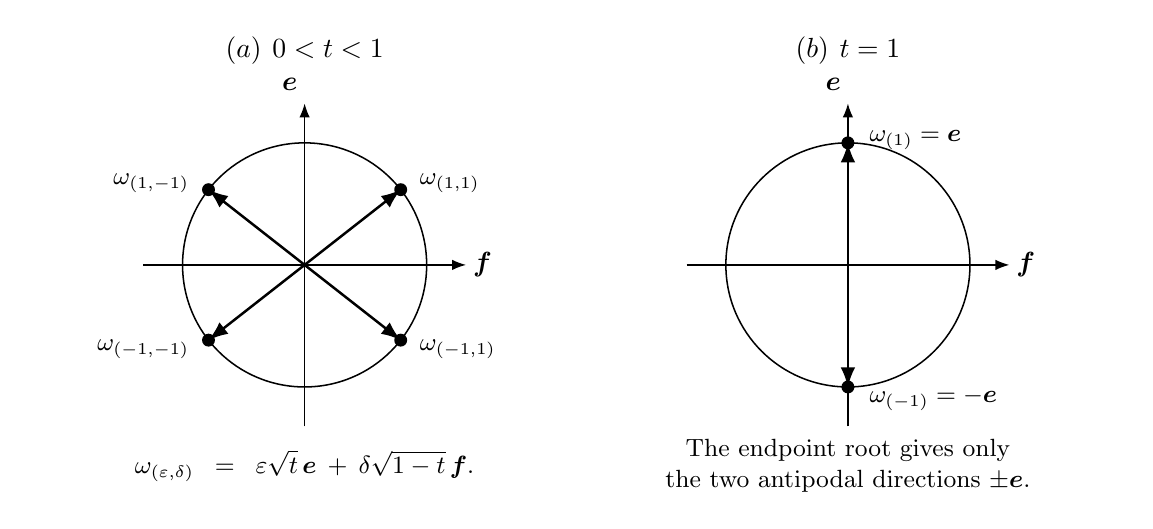
\begin{tikzpicture}[
  >=Latex,
  axis/.style={->, line width=0.45pt},
  circleline/.style={line width=0.55pt},
  vec/.style={->, line width=0.9pt},
  point/.style={circle, fill=black, inner sep=1.65pt},
  lab/.style={font=\small},
  title/.style={font=\normalsize\bfseries},
  note/.style={font=\small}
]

% Parameters
\def\R{1.55}
\def\ax{2.05}
\def\troot{0.38}
\pgfmathsetmacro{\x}{sqrt(\troot)}
\pgfmathsetmacro{\y}{sqrt(1-\troot)}

% Panel macro: axes + circle
\newcommand{\basecircle}[2]{%
  \begin{scope}[shift={(#1,#2)}]
    \draw[circleline] (0,0) circle (\R);
    \draw[axis] (-\ax,0) -- (\ax,0) node[right=-1pt] {$\bm f$};
    \draw[axis] (0,-\ax) -- (0,\ax) node[above left=1pt and -1pt] {$\bm e$};
  \end{scope}
}

% Left panel: 0<t<1
\node[title] at (-3.45,2.72) {$(a)$ $0<t<1$};
\basecircle{-3.45}{0}
\begin{scope}[shift={(-3.45,0)}]
  % vectors: omega = epsilon sqrt(t) e + delta sqrt(1-t) f
  % coordinates in drawing: horizontal=f=y, vertical=e=x
  \draw[vec] (0,0) -- ({\y*\R},{\x*\R});
  \draw[vec] (0,0) -- ({-\y*\R},{\x*\R});
  \draw[vec] (0,0) -- ({\y*\R},{-\x*\R});
  \draw[vec] (0,0) -- ({-\y*\R},{-\x*\R});
  \node[point] at ({\y*\R},{\x*\R}) {};
  \node[point] at ({-\y*\R},{\x*\R}) {};
  \node[point] at ({\y*\R},{-\x*\R}) {};
  \node[point] at ({-\y*\R},{-\x*\R}) {};
  \node[lab, anchor=west] at ({\y*\R+0.12},{\x*\R+0.08}) {$\omega_{(1,1)}$};
  \node[lab, anchor=east] at ({-\y*\R-0.12},{\x*\R+0.08}) {$\omega_{(1,-1)}$};
  \node[lab, anchor=west] at ({\y*\R+0.12},{-\x*\R-0.12}) {$\omega_{(-1,1)}$};
  \node[lab, anchor=east] at ({-\y*\R-0.12},{-\x*\R-0.12}) {$\omega_{(-1,-1)}$};
  % dashed projection on first quadrant
%  \draw[dashed, line width=0.4pt] ({\y*\R},{\x*\R}) -- ({\y*\R},0);
%  \draw[dashed, line width=0.4pt] ({\y*\R},{\x*\R}) -- (0,{\x*\R});
%  \node[note, anchor=west] at ({\y*\R+0.12},{0.5*\x*\R}) {$\varepsilon\sqrt t$};
%  \node[note, anchor=south] at ({0.5*\y*\R},{\x*\R+0.06}) {$\delta\sqrt{1-t}$};
\end{scope}
\node[note, text width=6.8cm, align=center] at (-3.45,-2.55)
  {$\displaystyle \omega_{(\varepsilon,\delta)}=\varepsilon\sqrt t\,\bm e+\delta\sqrt{1-t}\,\bm f.$};

% Right panel: t=1
\node[title] at (3.45,2.72) {$(b)$ $t=1$};
\basecircle{3.45}{0}
\begin{scope}[shift={(3.45,0)}]
  \draw[vec] (0,0) -- (0,\R);
  \draw[vec] (0,0) -- (0,-\R);
  \node[point] at (0,\R) {};
  \node[point] at (0,-\R) {};
  \node[lab, anchor=west] at (0.15,\R+0.04) {$\omega_{(1)}=\bm e$};
  \node[lab, anchor=west] at (0.15,-\R-0.16) {$\omega_{(-1)}=-\bm e$};
\end{scope}
\node[note, text width=6.8cm, align=center] at (3.45,-2.55)
  {The endpoint root gives only the two antipodal directions $\pm\bm e$.};

\end{tikzpicture}

\caption{Admissible scattering directions associated with one admissible root $t\in (0,1]$ of the quadratic polynomial $Q(t)$.}
\label{fig:vectors}
\end{figure}

\begin{remark}
The variable $t=({\bm\omega}\cdot{\bm e})^2$
has a simple geometric interpretation: it is the squared projection of the scattering direction onto the distinguished direction ${\bm e}={\bm E}_{\perp}/|{\bm E}_{\perp}|$
on the collision circle $S^2\cap{\bm B}^{\perp}$. Hence, the quadratic equation $Q(t)=0$ determines the admissible positions of ${\bm\omega}$ on this circle.
\end{remark}
By Theorem~\ref{quadraticreduction}, the cardinality of the collision manifold is determined entirely by the location of the roots of $Q$ relative to the interval $(0,1]$.
To express neatly the number of elements of the collision manifold,
let
\[
N_{\mathrm{int}}=\#\{t\in(0,1):Q(t)=0\},
\]
and let
\[
N_{\mathrm{end}}=
\begin{cases}
1, & Q(1)=0,\\
0, & Q(1)\neq0.
\end{cases}
\]
Then 
\[
{\bm E}\times{\bm B}\neq0 \Rightarrow \# \mathcal{X}_\mathrm{COM}(M,{\bm E}, {\bm B})= 4N_{\mathrm{int}}+2N_{\mathrm{end}}.
\]
Since $Q$ is quadratic, one has $N_{\mathrm{int}}\in\{0,1,2\}$.
Therefore, the possible finite numbers of admissible collision states are
\[
0,\ 2,\ 4,\ 6,\ 8.
\]
Figure~\ref{fig:cardinality} illustrates the possible geometric configurations.




\begin{figure}[ht!]
\centering
% TikZ input file: possible cardinalities of the collision manifold
% Required packages in main document:
% \usepackage{tikz}
% \usetikzlibrary{arrows.meta,calc}
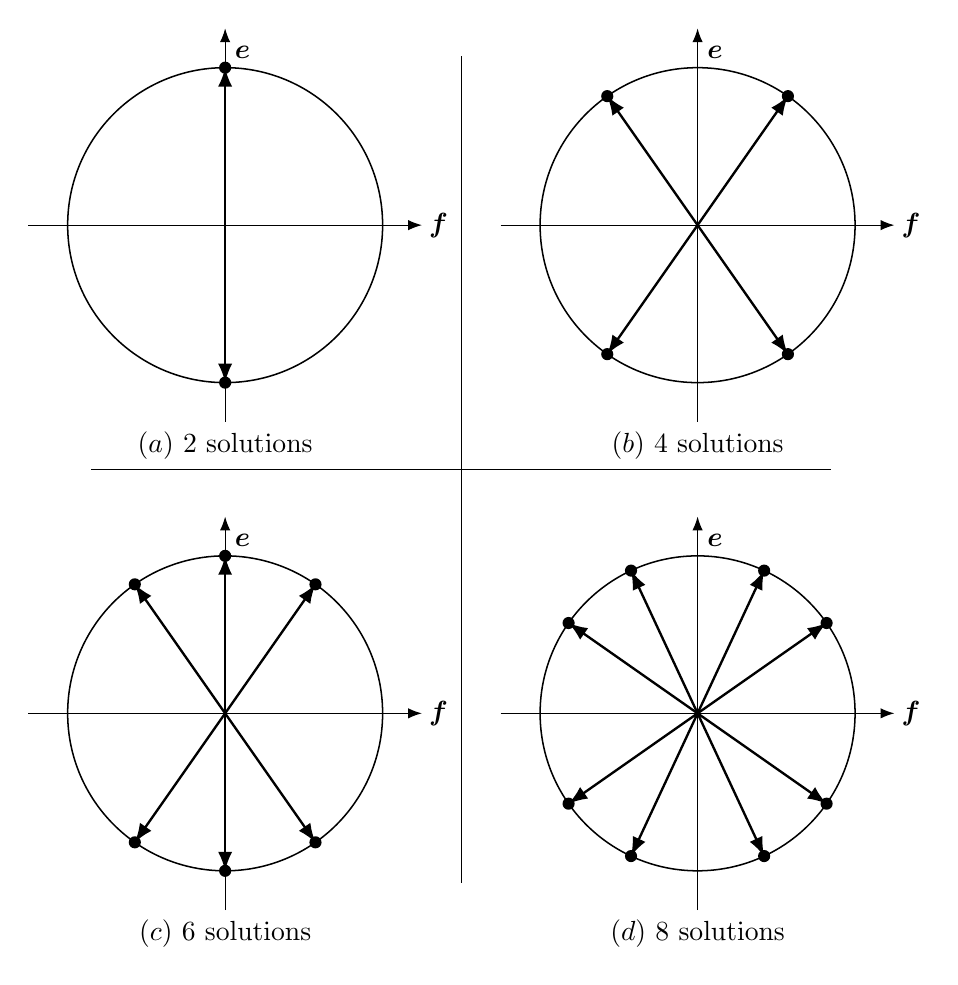
\begin{tikzpicture}[
  >=Latex,
  axis/.style={->, line width=0.45pt},
  circleline/.style={line width=0.55pt},
  vec/.style={->, line width=0.85pt},
  point/.style={circle, fill=black, inner sep=1.55pt},
  title/.style={font=\normalsize},
]
\def\R{2}
\def\ax{2.5}
\def\sepX{6}
\def\sepY{6.20}

\newcommand{\panel}[4]{%
  % #1,#2 shift; #3 title; #4 comma-separated angles in degrees measured from f-axis
  \begin{scope}[shift={(#1,#2)}]
    \node[title] at (0,-2.8) {#3};
    \draw[circleline] (0,0) circle (\R);
    \draw[axis] (-\ax,0) -- (\ax,0) node[right=-1pt] {$\bm f$};
    \draw[axis] (0,-\ax) -- (0,\ax);
    \node at (0.22,2.2) {$\bm e$};
    \foreach \ang in {#4}{
      \draw[vec] (0,0) -- ({\R*cos(\ang)},{\R*sin(\ang)});
      \node[point] at ({\R*cos(\ang)},{\R*sin(\ang)}) {};
    }
  \end{scope}
}

% Angles are drawn in the (f,e)-plane: 0 deg is +f, 90 deg is +e.
\panel{-\sepX/2}{\sepY/2}{$(a)$ $2$ solutions}{90,270}
\panel{\sepX/2}{\sepY/2}{$(b)$ $4$ solutions}{55,125,235,305}
\panel{-\sepX/2}{-\sepY/2}{$(c)$ $6$ solutions}{90,55,125,235,305,270}
\panel{\sepX/2}{-\sepY/2}{$(d)$ $8$ solutions}{35,65,115,145,215,245,295,325}

% separators
\draw[line width=0.35pt] (0,-5.25) -- (0,5.25);
\draw[line width=0.35pt] (-4.7,0) -- (4.7,0);

\end{tikzpicture}

\caption{Typical configurations of the collision manifold
$\mathcal X_{\mathrm{COM}}(M,\bm E,\bm B)$ in the generic case
$\bm E\times\bm B\neq0$. The black arrows represent the admissible
scattering directions $\bm\omega\in S^2\cap\bm B^\perp$. In the of 8 solutions case, there are two roots of $Q(t)$ in the interval $(0,1)$, each giving rise to a set of 4 vectors $\bm\omega_{(\varepsilon,\delta)}$. By Corollary~\ref{nonemptycondition}, the generic
cardinalities of admissible configuration sets are $4$ and $8$.}
\label{fig:cardinality}
\end{figure}

\begin{remark}
The multiplicities in the classification have a direct geometric origin. Each root $t\in(0,1)$ fixes the absolute value of the projection of ${\bm\omega}$ onto ${\bm e}$, but leaves two choices for the sign of this projection and two choices for the sign of the orthogonal component. Thus, each interior root gives four points on the collision circle. In contrast, the endpoint root $t=1$ gives only the two antipodal points $\pm{\bm e}$. 
\end{remark}

In the next theorem we characterize the cardinality of the collision manifold in terms of inequalities on the conserved quantities ${\bm E}$, ${\bm B}$. 



\begin{theorem}\label{cardinalitytheorem}
Assume that 
\[
{\bm E}\times{\bm B}\neq0
\]
 and recall the definitions of $A,C,D$ in~\eqref{CD},~\eqref{A}. 
The cardinality of the collision manifold is as follows.

If $D<A$, then
\[
\#\mathcal X_{\mathrm{COM}}(M,{\bm E},{\bm B})
=
\begin{cases}
0, & C<2\sqrt{AD},\\
4, & C=2\sqrt{AD},\ \text{or}\ C>A+D\\
6, & C=A+D,\\
8, & 2\sqrt{AD}<C<A+D.
\end{cases}
\]


If $D\geq A$, then
\[
\#\mathcal X_{\mathrm{COM}}(M,{\bm E},{\bm B})
=
\begin{cases}
0, & C<A+D,\\
2, & C=A+D,\\
4, & C>A+D.
\end{cases}
\]
\end{theorem}

\begin{proof}
For $t>0$~\eqref{Qequation}
is equivalent to
\[
C=At+\frac{D}{t}.
\]
Define
\[
f(t):=At+\frac{D}{t},
\qquad 0<t\le1.
\]
The admissible values of $t$ are precisely the intersections of the graph of $f$ with the horizontal line of height $C$.
Since
\[
f'(t)=A-\frac{D}{t^2},
\]
the unique critical point of $f$ on $(0,\infty)$ is $t_*=\sqrt{D/A}$. 
If $D<A$, then $
t_*\in(0,1)$, $f(t_*)=2\sqrt{AD}$, $f(1)=A+D$
and $f$ has a minimum at $t=t_*$. Hence there are no admissible roots if $C<2\sqrt{AD}$, one interior double root if $C=2\sqrt{AD}$, two interior roots if $2\sqrt{AD}<C<A+D$, one interior root together with the endpoint root $t=1$ if $C=A+D$, and one interior root if $C>A+D$. Since each interior root gives four points of $\mathcal X_{\mathrm{COM}}$, while the endpoint root gives two points, the claimed cardinalities follow.
If $D\geq A$, then $t_*>1$, so $f$ is decreasing on $(0,1]$, with $
f(1)=A+D$.
Thus there are no admissible roots if $C<A+D$, the only admissible root is $t=1$ if $C=A+D$, and there is exactly one interior root if $C>A+D$. This completes the proof.
\end{proof}

\begin{corollary}\label{nonemptycondition}
Assume that ${\bm E}\times{\bm B}\neq0$. Then
\begin{equation}\label{emptyX}
\mathcal X_{\mathrm{COM}}(M,{\bm E},{\bm B})\neq\emptyset
\iff
C\ge
\begin{cases}
2\sqrt{AD}, & D<A,\\
A+D, & D\ge A.
\end{cases}
\end{equation}
Moreover, the cardinality of $\mathcal X_{\mathrm{COM}}(M,{\bm E},{\bm B})$ changes only on the hypersurfaces
\[
C=2\sqrt{AD},
\qquad
C=A+D.
\]
In particular, away from these hypersurfaces the generic finite cardinalities are
\[
\#\mathcal X_{\mathrm{COM}}(M,{\bm E},{\bm B})\in\{0,4,8\}.
\]
\end{corollary}
\begin{remark}
When $A=0$, the inequality in~\eqref{emptyX} reduces to
$
C\ge D,
$
which is precisely the condition obtained in Theorem~\ref{exceptionalcase}
for the collision manifold to be nonempty in the exceptional case
${\bm E}\times{\bm B}=0$.
\end{remark}


\section{Reconstruction of the admissible collision states}\label{reconstructionSEC}
Theorem \ref{cardinalitytheorem} determines the number of admissible collision states for any prescribed conserved quantities. The next theorem shows how to uniquely reconstruct an admissible collision state from each element of the collision manifold, thereby completing the solution of the collision problem.
\begin{theorem}\label{reconstruction}
Assume $\mathcal X_{\mathrm{COM}}(M,{\bm E},{\bm B})\neq\emptyset$. 
Given $(\bm \omega,\alpha)\in\mathcal X_{\mathrm{COM}}(M,{\bm E},{\bm B})$, define the vectors ${\bm U}, {\bm V}$ from the conserved quantities ${\bm E},{\bm B}$ by
\begin{subequations}\label{final}
\begin{equation}\label{final1}
{\bm U}=\frac2M\left({\bm E}-({\bm E}\cdot {\bm \omega}){\bm \omega}\right)+\frac{M}{2m^2}({\bm E}\cdot {\bm \omega}){\bm \omega},\quad
{\bm V}= \frac1\kappa {\bm B}\times {\bm \omega}+\alpha {\bm \omega},
\end{equation}
Then the admissible four-momenta and spin vectors in the COM frame are given by
\begin{equation}\label{final3}
p=(M/2, \kappa\, {\bm \omega}),\quad q=(M/2,-\kappa\,\bm \omega),
\end{equation}
\begin{equation}\label{final4}
{\bm s}=\frac12({\bm U}+{\bm V}),\ s^0=\frac{2}{M}{\bm p}\cdot{\bm s},\quad \quad{\bm r}=\frac12({\bm U}-{\bm V}),\ r^0=\frac{2}{M}{\bm q}\cdot{\bm r},
\end{equation}
and the admissible spin tensors are given by
\begin{equation}
\phi=\frac{1}{\sqrt{2}m}*(p\wedge s),\quad \psi=\frac{1}{\sqrt{2}m}*(q\wedge r).
\end{equation}
\end{subequations}
\end{theorem}

\begin{thebibliography}{99}
\bibitem[Groot]{Groot} S.~R.~de Groot, W.~A.~van Leeuwen Ch.~G.~van Weert: {\it Relativistic kinetic theory. Principles and Applications}. North-Holland Publishing Company (1980)
\end{thebibliography}
\end{document}
